%--------------------------------------------------------------------------------------------------%
\chapter{PERANCANGAN}
\label{chap:3}
%--------------------------------------------------------------------------------------------------%

Bab ini berisi perancangan arsitektur konversi, ontologi KG yang dihasilkan, dikaitkan dengan
\textit{competency questions}. \textit{Competency questions} harus diperjelas untuk dijadikan
landasan ontologi KG. KG yang dihasilkan oleh sistem konversi, digabung dengan ontologi yang sudah
dirancang harus dapat menjawab semua pertanyaan pada \textit{competency questions}.

%--------------------------------------------------------------------------------------------------%
\section{Arsitektur Sistem Konversi}
\label{sec:arsitektur-sistem-konversi}
%--------------------------------------------------------------------------------------------------%

\begin{figure}
  \centering
  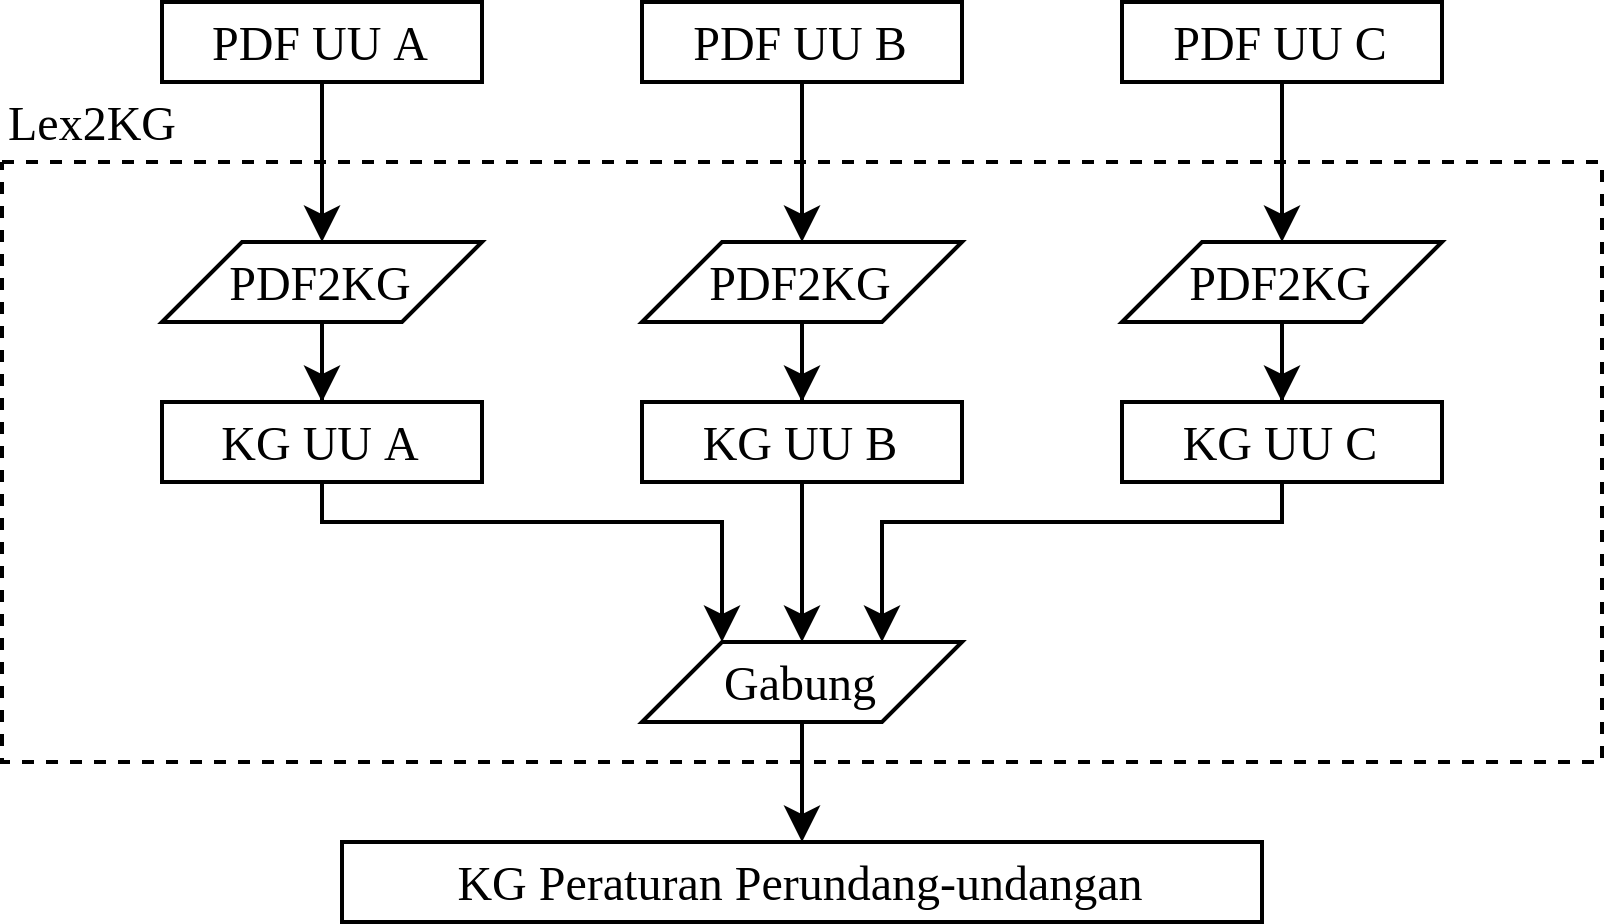
\includegraphics[scale=0.35]{pictures/lex2kg.png}
  \caption{Arsitektur Lex2KG}
  \label{fig:lex2kg}
\end{figure}

Lex2KG melakukan konversi masing-masing PDF \legal menjadi KG menggunakan modul PDF2KG kemudian KG
dari masing-masing PDF digabung dan dikeluarkan sebagai satu KG, seperti yang terlihat pada
\pic~\ref{fig:lex2kg}. KG dikeluarkan dalam format RDF Turtle di mana setiap barisnya merupakan
\textit{triple} yang terdapat pada KG, sehingga penggabungan KG dapat dilakukan dengan mudah yaitu
dengan menggabungkan baris-baris tersebut ke dalam satu berkas. 

\begin{figure}
  \centering
  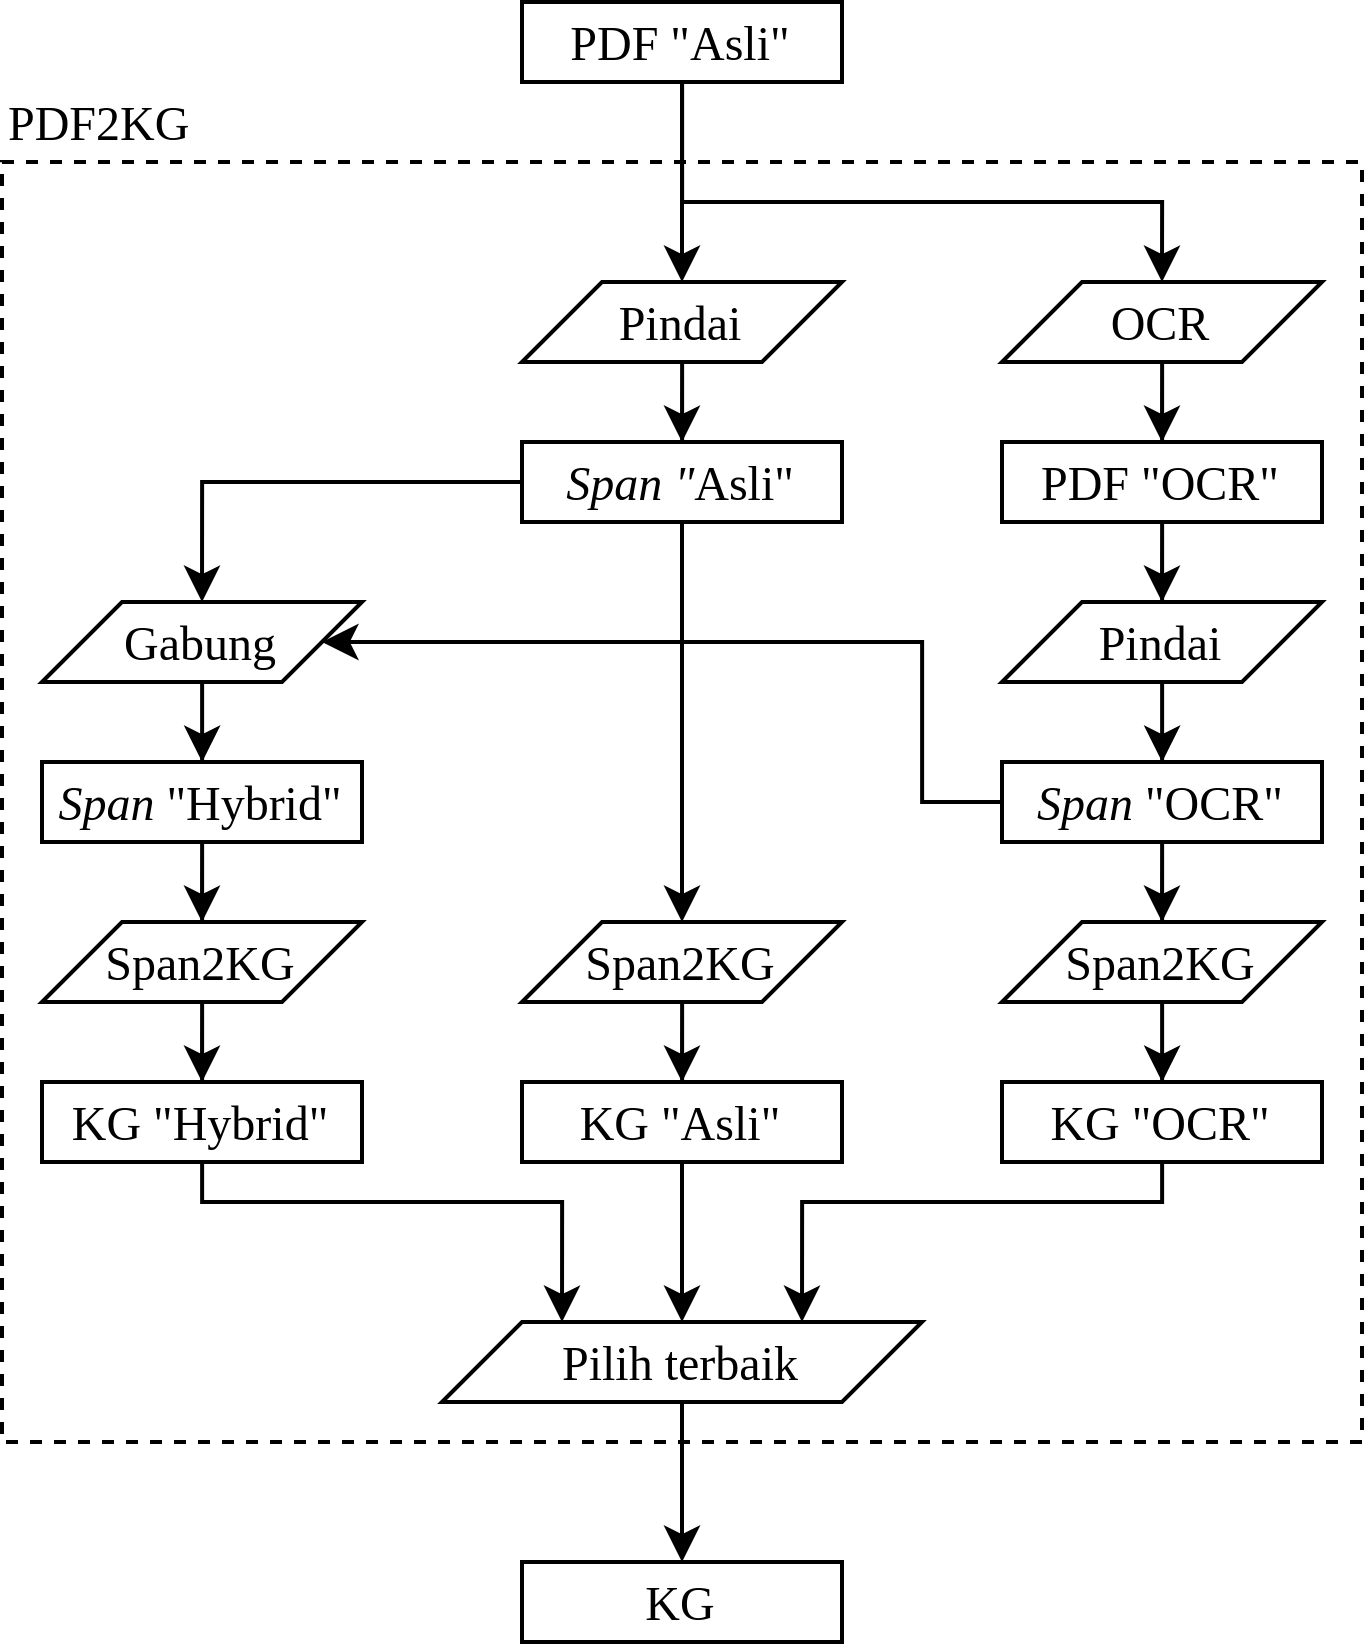
\includegraphics[scale=0.35]{pictures/pdf2kg.png}
  \caption{Arsitektur PDF2KG}
  \label{fig:pdf2kg}
\end{figure}

PDF2KG memiliki arsitektur seperti yang ditunjukan pada \pic~\ref{fig:pdf2kg}. Bagian
\textit{Optical Character Recognition} (OCR) bertanggung jawab untuk mengubah \textit{image-only}
PDF ("Asli) menjadi \textit{text-scannable} PDF ("OCR") dan menstandardisasi pemformatan semua PDF.
Selanjutnya kedua file PDF "Asli" dan "OCR" dipindai untuk mengekstrak teks beserta posisinya, yang
selanjutnya disebut \textit{span}. Kemudian \textit{span} "Asli" dan \textit{span} "OCR" digabung
untuk dibuat \textit{span} "Hybrid". Kemudian PDF2KG membuat tiga versi KG dari masing-masing
\textit{span} "Asli", "OCR", dan "Hybrid" menggunakan Span2KG untuk dipilih satu KG terbaik yang
akan dikeluarkan, di mana KG terbaik adalah KG dengan \textit{triple} terbanyak. Walaupun KG dengan
\textit{triple} terbanyak merupakan KG yang terbaik, karena penulis tidak memiliki fungsi evaluasi
untuk mengetahui kualitas KG, penulis menggunakan asumsi naif berdasarkan pengamatan subyektif
penulis, bahwa KG dengan \textit{triple} terbanyak merupakan KG yang memuat informasi terbanyak dari
PDF.

\begin{figure}
  \centering
  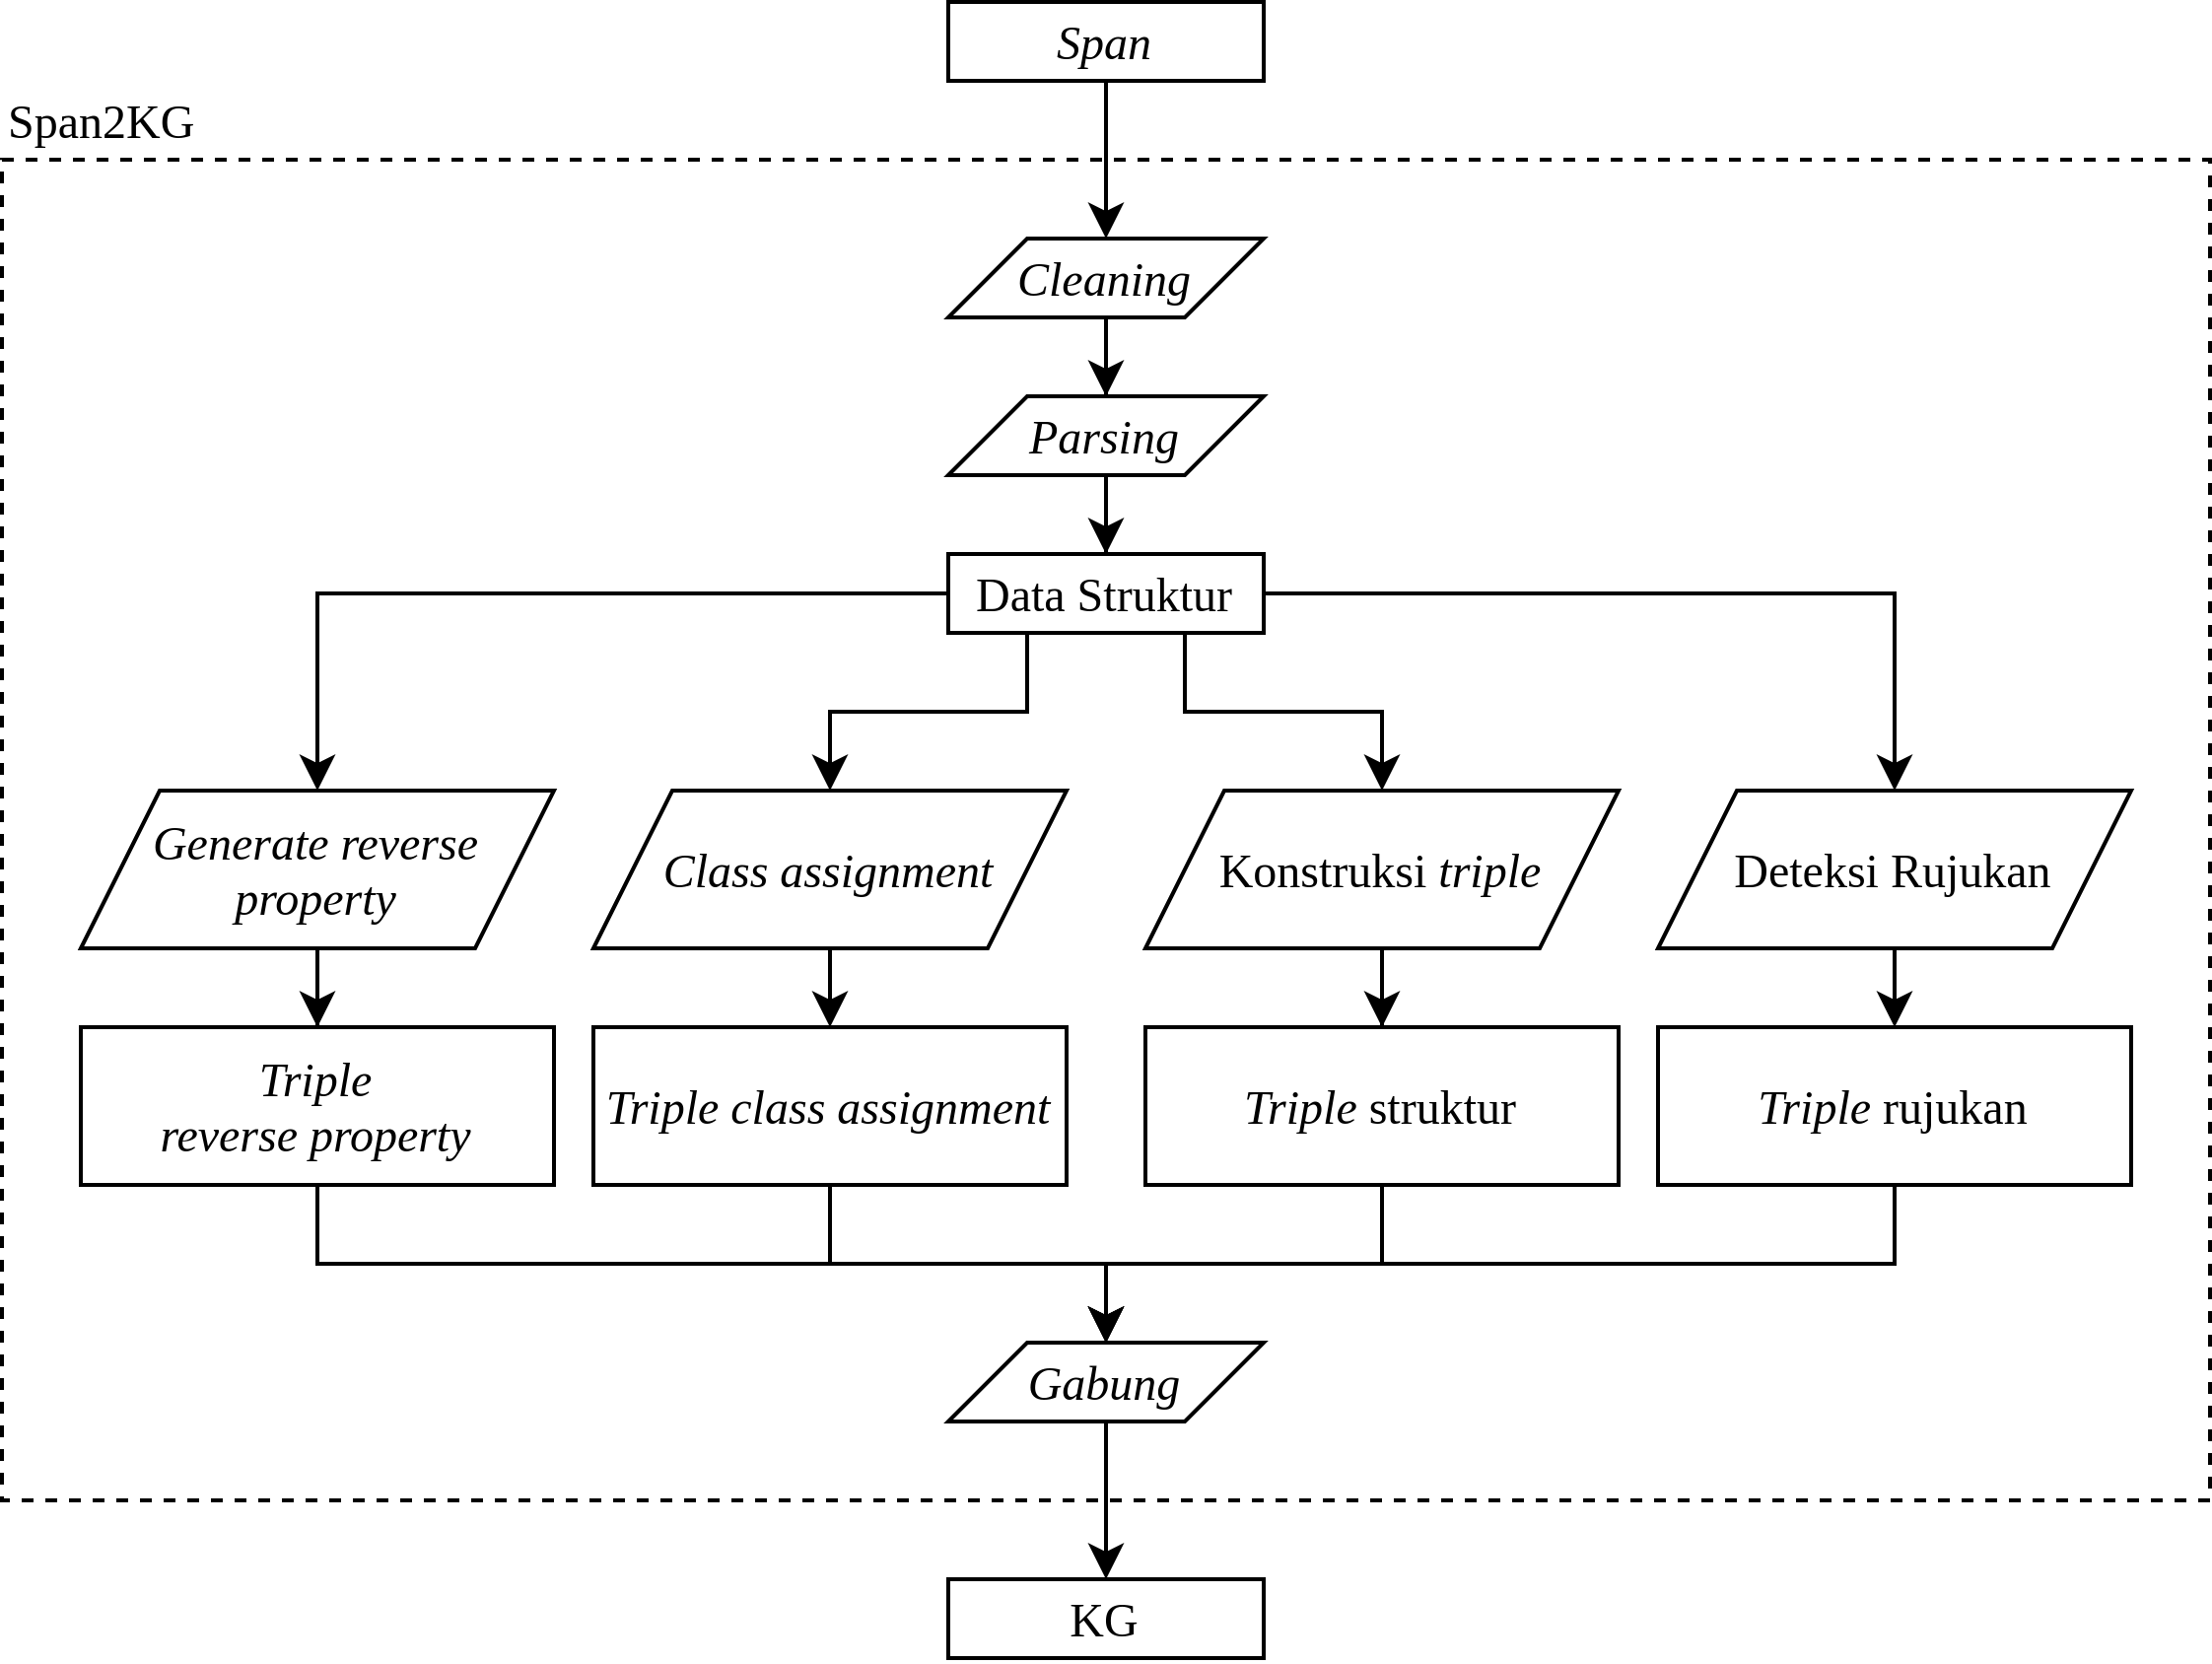
\includegraphics[width=\textwidth]{pictures/span2kg.png}
  \caption{Arsitektur Span2KG}
  \label{fig:span2kg}
\end{figure}

Pada PDF2KG terdapat modul Span2KG yang melakukan konversi \textit{span} menjadi KG dengan
arsitektur seperti yang dijelaskan pada \pic~\ref{fig:span2kg}. Pada Span2KG \textit{span} input
yang terdeteksi sebagai konten yang tidak relevan, seperti \textit{header} dan \textit{footer} yang
berulang, akan disaring. \textit{Clean span} yang dihasilkan, kemudian dilakukan \textit{parsing}
sehingga menjadi data struktur peraturan. Kemudian data tersebut dibuat menjadi \textit{triple}
struktur, \textit{class assignment}, dan \textit{reverse property} sesuai yang didefinisikan pada
ontologi. \textit{Reverse property} merupakan properti yang memiliki sifat kebalikan dari suatu
properti lain, untuk mempermudah \textit{query}. Selain itu, pada data struktur juga dilakukan
deteksi rujukan yang kemudian menghasilkan \textit{triple} rujukan. Pada tahap akhir, Span2KG
menggabungkan semua \textit{triple} tersebut dan dikeluarkan sebagai KG. Pada proses konstruksi KG
ini, \textit{triple} yang dihasilkan akan mengikuti spesifikasi yang diberikan pada ontologi.

%--------------------------------------------------------------------------------------------------%
\section{\textit{Competency Questions}}
\label{sec:competency-questions}
%--------------------------------------------------------------------------------------------------%

\textit{Competency questions} perlu didefinisikan untuk dijadikan landasan perangancan ontologi KG
yang dihasilkan. Setiap \textit{competency question} harus dapat dijawab oleh KG yang dihasilkan
dengan membuktikan SPARQL \textit{query} yang bersesuaian dengan pertanyaan tersebut mengembalikan
hasil yang benar. Pada penelitian ini, \textit{competency questions} disusun dari
pertanyaan-pertanyaan yang menurut peneliti dan dosen pembimbing seharusnya dapat dijawab
berdasarkan informasi yang diberikan pada PDF dari informasi strukturnya, serta data-data yang dapat
diekstrak dengan pemrograman deterministik seperti \textit{regular expression}, bukan seperti
\textit{natural language processing} dan \textit{machine learning}. Beberapa konsep \legal memiliki
konteks spesifik untuk Indonesia, oleh karena itu, pembuatan ontologi akan dilakukan berdasarkan UU
10/2004 tentang pembentukan \legal. \tab~\ref{tab:competency-questions} merupakan daftar
\textit{competency questions} yang didefinisikan pada penelitian ini. Pada \textit{competency
question} terdapat banyak pertanyaan yang terkait dengan UU 11/2020 tentang Cipta Kerja. Hal ini
disebabkan UU Cipta Kerja memuat jenis informasi yang relatif lengkap. Sebagai contoh, UU Cipta
Kerja melakukan ketiga jenis amendemen yaitu penyisipan, pengubahan, dan penghapusan.

\begin{longtable}[l]{|p{0.05\textwidth} | p{0.95\textwidth}|}
  \hline
  \textbf{No.} & \textbf{Pertanyaan}                                                                                                         \\ \hline \endhead
  1            & Deskripsikan UU Cipta Kerja.                                                                                                \\ \hline
  2            & Tampilkan semua pasal dari UU Cipta Kerja.                                                                                  \\ \hline
  3            & Tampilkan teks dari Pasal 2 Ayat 1 UU Cipta Kerja.                                                                          \\ \hline
  4            & Tampilkan semua pasal yang terdapat pada Bab 2 UU Cipta Kerja.                                                              \\ \hline
  5            & Tampilkan ayat yang mengandung teks "kompensasi" dan "buruh" yang disisipkan oleh  UU Cipta Kerja.                          \\ \hline
  6            & Tampilkan komponen dari UU Cipta Kerja yang menyisipkan pasal ke UU Ketenagakerjaan dan pula teks dari pasal tersebut.      \\ \hline
  7            & Tampilkan komponen dari UU Cipta Kerja yang mengubah pasal UU Ketenagakerjaan dan tambilkan sebelum dan setelah pengubahan. \\ \hline
  8            & Tampilkan komponen dari UU Cipta Kerja yang menghapus pasal UU Ketenagakerjaan dan pula teks dari pasal tersebut.           \\ \hline
  9            & Tampilkan peraturan yang paling banyak diamendemen oleh UU Cipta Kerja.                                                     \\ \hline
  10           & Tampilkan banyaknya penyisipan, pengubahan, dan penghapusan pasal yang dilakukan UU Cipta Kerja terhadap UU lain.                 \\ \hline
  11           & Tampilkan pasal pada UU Ketenagakerjaan setelah dilakukan oleh UU Cipta Kerja.                                              \\ \hline
  12           & Tampilkan pasal pada UU Cipta Kerja yang tidak melakukan amendemen.                                                         \\ \hline
  13           & Tampilkan pasal pada UU Cipta Kerja yang menghapus pasal yang disahkan setelah tahun 2001.                                  \\ \hline
  14           & Tampilkan pasal yang disisipkan oleh UU Cipta Kerja dan rujukan yang terdapat pada pasal jika ada.                          \\ \hline
  15           & Tampilkan semua peraturan serta peraturan yang ditimbangnya.                                                                \\ \hline
  16           & Tampilkan 10 peraturan dengan pasal terbanyak.                                                                              \\ \hline
  17           & Tampilkan peraturan yang pernah diamendemen.                                                                                \\ \hline
  18           & Tampilkan 10 tempat terbanyak peraturan disahkan.                                                                           \\ \hline
  19           & Tampilkan 10 peraturan paling banyak ditimbang.                                                                             \\ \hline
  20           & Tampilkan semua peraturan yang melakukan amendemen dan banyaknya pasal yang amendemen oleh pasal tersebut.                  \\ \hline
  21           & Tampilkan jumlah \textit{triple} tentang struktur peraturan.                                                                \\ \hline
  22           & Tampilkan jumlah \textit{triple} tentang metadata peraturan.                                                                \\ \hline
  23           & Tampilkan jumlah \textit{triple} tentang teks peraturan.                                                                    \\ \hline
  24           & Tampilkan jumlah \textit{triple} tentang rujukan peraturan.                                                                 \\ \hline
  25           & Tampilkan jumlah \textit{triple} tentang amendemen peraturan.                                                               \\ \hline
  26           & Tampilkan jumlah \textit{triple} tentang \textit{class assignment}.                                                         \\ \hline
  27           & Tampilkan 5 peraturan dengan komponen terbanyak beserta jumlah komponennya.                                                 \\ \hline
  28           & Peraturan apa yang berlaku pada daerah X yang disahkan di tahun Y?                                                          \\ \hline
  29           & Apa relasi suatu peraturan dengan peraturan lain?                                                                           \\ \hline
  30           & Mana saja peraturan yang membahas tentang topik W atau X tapi bukan topik Y dan bukan Z?                                    \\ \hline
  31           & Apa isi dari Pasal X ayat (Y) huruf Z dari suatu \legal?                                                                    \\ \hline
  32           & Apa saja bab-bab yang terdapat pada peraturan X?                                                                            \\ \hline
  \caption{\textit{Competency questions}}
  \label{tab:competency-questions}
\end{longtable}


%--------------------------------------------------------------------------------------------------%
\section{\textit{Lex2KG Namespace}}
\label{sec:perancangan-uri}
%--------------------------------------------------------------------------------------------------%

Setiap entitas yang berbeda perlu diberikan URI yang berbeda. Penggabungan KG sangat umum dilakukan
karena secara struktur dapat dilakukan dengan mudah, dan dapat memperkuat data dari masing-masing
KG. KG memiliki entitas-entitas dengan URI yang unik, oleh karena itu saat menggabungkan sebuah KG A
dan sebuah KG B, entitas yang berbeda harus memiliki URI yang berbeda. Sebuah masalah dapat terjadi
apabila URI tidak dirancang dengan benar. Sebagai contoh, apabila terdapat entitas dari KG A dengan
URI \mono{https://example.org/trump} dengan maksud Donald Trump mantan presiden Amerika Serikat,
dan entitas dari KG B dengan URI yang sama dengan maksud permainan kartu Trump, saat kedua KG ini
digabung akan menjadi informasi yang berkontradiksi. Oleh karena itu, pada umumnya digunakan
\textit{namespace} yang berbeda untuk masing-masing KG. Sebagai contoh, dengan KG A menggunakan
\textit{namespace} \mono{https://kga.org} dan KG B menggunakan \textit{namespace}
\mono{https://kgb.org}, dua entitas yang sebelumnya berkontradiksi akan memiliki URI yang berbeda
yaitu \mono{https://kga.org/trump} dan \mono{https://kgb.org/trump}.

Pada penelitian ini digunakan \textit{namespace} \mono{https://example.org/lex2kg/}.
\textit{Namespace} yang digunakan oleh Lex2KG dapat dikonfigurasi. \tab~\ref{tab:prefixes} adalah
daftar \textit{prefix} dan notasi singkatnya pada yang akan digunakan pada selanjutnya.

\begin{table}
  \centering
  \begin{tabular}{|l|l|l|} \hline
    notasi singkat & \textit{prefix}                                             \\ \hline \hline
    \texttt{:}     & \texttt{https://example.org/lex2kg/}                        \\ \hline
    \texttt{o:}    & \texttt{https://example.org/lex2kg/ontology/}               \\ \hline
    \texttt{jp:}   & \texttt{https://example.org/lex2kg/ontology/jenisPeraturan} \\ \hline
    \texttt{uu:}   & \texttt{https://example.org/lex2kg/uu/}                     \\ \hline
  \end{tabular}
  \caption{\textit{Prefix} dan notasi singkatnya}
  \label{tab:prefixes}
\end{table}

%--------------------------------------------------------------------------------------------------%
\section{Perancangan \textit{Class} dan URI \textit{Class}}
\label{sec:perancangan-uri-class}
%--------------------------------------------------------------------------------------------------%

Huruf pertama dari nama \textit{class} dibuat kapital mengikuti konvensi RDF \citep{rdf_spec}.
\textit{Class} Lex2KG terdiri dari \textit{Class} komponen \legal seperti \mono{o:Bab} dan
\textit{Class} \legal sendiri yaitu \mono{o:Peraturan}. \tab~\ref{tab:class} adalah semua URI
\textit{class} Lex2KG beserta URI dan deskripsinya.

\begin{longtable}[l]{|p{0.22\textwidth}|p{0.78\textwidth}|}
  \hline
  \textbf{URI Class}        & \textbf{Deskripsi}                                                                              \\ \hline \endhead
  \texttt{o:Peraturan}      & \Legal                                                                                          \\ \hline
  \texttt{o:DaftarBab}      & Daftar satu atau lebih bab                                                                      \\ \hline
  \texttt{o:Bab}            & Bab                                                                                             \\ \hline
  \texttt{o:DaftarBagian}   & Daftar satu atau lebih bagian                                                                   \\ \hline
  \texttt{o:Bagian}         & Bagian                                                                                          \\ \hline
  \texttt{o:DaftarParagraf} & Daftar satu atau lebih paragraf                                                                 \\ \hline
  \texttt{o:Paragraf}       & Paragraf                                                                                        \\ \hline
  \texttt{o:DaftarPasal}    & Daftar satu atau lebih pasal                                                                    \\ \hline
  \texttt{o:Pasal}          & Pasal                                                                                           \\ \hline
  \texttt{o:VersiPasal}     & Versi dari sebuah pasal. Sebuah pasal dapat memiliki satu atau lebih versi dari hasil amendemen \\ \hline
  \texttt{o:DaftarAyat}     & Daftar satu atau lebih ayat                                                                     \\ \hline
  \texttt{o:Ayat}           & Ayat                                                                                            \\ \hline
  \texttt{o:DaftarHuruf}    & Daftar satu atau lebih huruf atau nomor                                                         \\ \hline
  \texttt{o:Huruf}          & Huruf atau nomor                                                                                \\ \hline
  \texttt{o:Menimbang}      & Hal yang ditimbang oleh suatu peraturan                                                         \\ \hline
  \texttt{o:Mengingat}      & Hal yang diingat oleh suatu peraturan                                                           \\ \hline
  \texttt{o:Segmen}         & Segmen teks. Dapat memiliki rujukan ke suatu komponen peraturan                                 \\ \hline
  \caption{Class Lex2KG}
  \label{tab:class}
\end{longtable}

%--------------------------------------------------------------------------------------------------%
\section{Perancangan Jenis Peraturan dan URI Jenis Peraturan}
\label{sec:perancangan-jenis-peraturan}
%--------------------------------------------------------------------------------------------------%

Setiap peraturan memiliki URI yang berbeda, yang akan digunakan oleh entitas sebagai prefix.
\tab~\ref{tab:uri-peraturan} adalah jenis \legal yang diimplementasi pada penelitian ini beserta URI
nya. Variabel akan ditandai dengan kurung kurawal ``\mono{\{\}}''. Diluar jenis peraturan yang
diimplementasi URI nya, ontologi Lex2KG juga memiliki resource sendiri yang mendefinisikan jenis
dari \legal terdaftar pada \tab~\ref{tab:uri-jenis-peraturan}. Beberapa jenis peraturan adalah
spesifik terhadapa kasus di Indonesia, seperti pembagian daerah yurisdiksi dan nama-nama daerah yang
hanya terdapat di Indonesia, sehingga diperlukan perancagan khusus URI untuk kasus Indonesia tersebut.

\begin{longtable}[l]{|p{0.2\textwidth}|p{0.55\textwidth}|p{0.25\textwidth}|}
  \hline
  \textbf{Peraturan}                    & \textbf{URI}                                            & \textbf{Penjelasan variabel}               \\ \hline \endhead
  Undang-Undang Dasar 1945              & \texttt{:uud}                                           &                                            \\ \hline
  Undang-Undang                         & \texttt{:uu/\{thn\}/\{nmr\}}                            & \makecell[l]{\texttt{thn}: tahun peraturan \\\texttt{nmr}: nomor peraturan} \\ \hline
  Peraturan Pemerintah                  & \texttt{:pp/\{thn\}/\{nmr\}}                            & \makecell[l]{\texttt{thn}: tahun peraturan \\\texttt{nmr}: nomor peraturan} \\\hline
  Peraturan Daerah Provinsi DKI Jakarta & \texttt{:perda\_provinsi\_dki\_jakarta/\{thn\}/\{nmr\}} & \makecell[l]{\texttt{thn}: tahun peraturan \\\texttt{nmr}: nomor peraturan} \\\hline
  Peraturan Gubernur DKI Jakarta        & \texttt{:pergub\_dki\_jakarta/\{thn\}/\{nmr\}}          & \makecell[l]{\texttt{thn}: tahun peraturan \\\texttt{nmr}: nomor peraturan} \\\hline
  Peraturan Walikota Malang             & \texttt{:perwali\_malang/\{thn\}/\{nmr\}}               & \makecell[l]{\texttt{thn}: tahun peraturan \\\texttt{nmr}: nomor peraturan} \\\hline
  \caption{Konstruksi URI untuk \legal}
  \label{tab:uri-peraturan}
\end{longtable}

\begin{longtable}[l]{|p{0.5\textwidth}|p{0.5\textwidth}|}
  \hline
  \textbf{Jenis Peraturan}                     & \textbf{URI}                        \\ \hline \endhead
  Undang-Undang Dasar 1945                     & \texttt{jp:UUD}                     \\ \hline
  Ketetapan MPR                                & \texttt{jp:TapMPR}                  \\ \hline
  Undang-Undang                                & \texttt{jp:UU}                      \\ \hline
  Peraturan Pemerintah Pengganti Undang-Undang & \texttt{jp:Perpu}                   \\ \hline
  Peraturan Pemerintah                         & \texttt{jp:PP}                      \\ \hline
  Peraturan Presiden                           & \texttt{jp:Perpres}                 \\ \hline
  Peraturan Menteri                            & \texttt{jp:PeraturanMenteri}        \\ \hline
  Peraturan Daerah Provinsi                    & \texttt{jp:PerdaProvinsi}           \\ \hline
  Peraturan Gubernur                           & \texttt{jp:PeraturanGubernur}       \\ \hline
  Peraturan Daerah Kabupaten/Kota              & \texttt{jp:PerdaKabKota}            \\ \hline
  Peraturan Bupati/Walikota                    & \texttt{jp:PeraturanBupatiWalikota} \\ \hline
  Keputusan Presiden                           & \texttt{jp:KeputusanPresiden}       \\ \hline
  Keputusan Gubernur                           & \texttt{jp:KeputusanGubernur}       \\ \hline
  Keputusan Menteri                            & \texttt{jp:KeputusanMenteri}        \\ \hline
  Keputusan Bupati/Walikota                    & \texttt{jp:KeputusanBupatiWalikota} \\ \hline
  \caption{URI jenis \legal}
  \label{tab:uri-jenis-peraturan}
\end{longtable}

%--------------------------------------------------------------------------------------------------%
\section{Perancangan Komponen dan URI Komponen}
\label{sec:perancangan-komponen}
%--------------------------------------------------------------------------------------------------%

Setiap komponen dokumen merupakan entitas, dan memiliki URI. URI sebuah komponen didahului oleh
\textit{docURI} dan semua komponen yang mengatasinya. \tab~\ref{tab:uri-komponen} adalah jenis
komponen \legal beserta pola URI dan penjelasan variabelnya.

\begin{longtable}{|p{0.22\textwidth}|p{0.33\textwidth}|p{0.45\textwidth}|}
  \hline
  \textbf{Komponen}         & \textbf{URI}                            & \textbf{Penjelasan variabel}                                                                                                                             \\ \hline \endhead
  \texttt{o:DaftarBab}      & \texttt{\{docURI\}/bab}                 & \texttt{docURI}: URI peraturan yang mengatasi                                                                                                            \\ \hline
  \texttt{o:Bab}            & \texttt{\{daftarBabURI\}/\{no\}}        & \texttt{daftarBabURI}: URI \mono{o:DaftarBab} yang mengatasi                                                                                             \\
                            &                                         & \texttt{no}: Nomor bab                                                                                                                                   \\ \hline
  \texttt{o:DaftarBagian}   & \texttt{\{babURI\}/bagian}              & \texttt{babURI}: URI \mono{o:Bab} yang mengatasi                                                                                                         \\ \hline
  \texttt{o:Bagian}         & \texttt{\{daftarBagianURI\}/\{no\}}     & \texttt{daftarBagianURI}: URI \mono{o:DaftarBagian} yang mengatasi                                                                                       \\
                            &                                         & \texttt{no}: Nomor bagian                                                                                                                                \\ \hline
  \texttt{o:DaftarParagraf} & \texttt{\{bagianURI\}/paragraf}         & \texttt{bagianURI}: URI \mono{o:Bagian} yang mengatasi                                                                                                   \\ \hline
  \texttt{o:Paragraf}       & \texttt{\{daftarParagrafURI\}/\{no\}}   & \texttt{daftarParagrafURI}: URI \mono{o:DaftarBagian} yang mengatasi                                                                                     \\
                            &                                         & \texttt{no}: Nomor paragraf                                                                                                                              \\ \hline
  \texttt{o:DaftarPasal}    & \texttt{\{parentURI\}/daftarpasal}      & \texttt{parentURI}: URI \mono{o:Bab}, \mono{o:Bagian}, \mono{o:Paragraf} yang mengatasi                                                                  \\ \hline
  \texttt{o:Pasal}          & \texttt{\{docURI\}/pasal/\{no\}}        & \texttt{docURI}: URI peraturan yang mengatasi                                                                                                            \\
                            &                                         & \texttt{no}: Nomor pasal                                                                                                                                 \\ \hline
  \texttt{o:VersiPasal}     & \texttt{\{pasalURI\}/versi/\{tanggal\}} & \texttt{pasalURI}: URI \mono{o:Pasal} yang mengatasi                                                                                                     \\
                            &                                         & \texttt{tanggal}: Tanggal disahkan                                                                                                                       \\ \hline
  \texttt{o:DaftarAyat}     & \texttt{\{pasalURI\}/ayat}              & \texttt{pasalURI}: URI \mono{o:Pasal} yang mengatasi                                                                                                     \\ \hline
  \texttt{o:Ayat}           & \texttt{\{daftarAyatURI\}/\{no\}}       & \texttt{daftarAyatURI}: URI \mono{o:DaftarAyat} yang mengatasi                                                                                           \\
                            &                                         & \texttt{no}: Nomor ayat                                                                                                                                  \\ \hline
  \texttt{o:DaftarHuruf}    & \texttt{\{parentURI\}/huruf}            & \texttt{parentURI}: URI \mono{o:Ayat}, \mono{o:Huruf}, \mono{o:VersiPasal}, \mono{o:Menimbang}, \mono{o:Mengingat}, yang mengatasi                       \\ \hline
  \texttt{o:Huruf}          & \texttt{\{daftarHurufURI\}/\{id\}}      & \texttt{daftarHurufURI}: URI \mono{o:DaftarHuruf} yang mengatasi                                                                                         \\
                            &                                         & \texttt{id}: Nomor atau huruf                                                                                                                            \\ \hline
  \texttt{o:Menimbang}      & \texttt{\{docURI\}/menimbang}           & \texttt{docURI}: URI peraturan yang mengatasi                                                                                                            \\ \hline
  \texttt{o:Mengingat}      & \texttt{\{docURI\}/mengingat}           & \texttt{docURI}: URI peraturan yang mengatasi                                                                                                            \\ \hline
  \texttt{o:Segmen}         & \texttt{\{parentURI\}/\{name\}}         & \texttt{parentURI}: URI \mono{o:Ayat}, \mono{o:Huruf}, \mono{o:DaftarHuruf}, \mono{o:VersiPasal}, \mono{o:Menimbang}, \texttt{Mengingat}, yang mengatasi \\
                            &                                         & \texttt{name}: Nama teks                                                                                                                                 \\ \hline
  \caption{Konstruksi URI untuk komponen \legal}
  \label{tab:uri-komponen}
\end{longtable}

%--------------------------------------------------------------------------------------------------%
\section{Perancangan Properti dan URI Properti}
\label{sec:perancangan-uri-properti}
%--------------------------------------------------------------------------------------------------%

Properti menghubungkan subjek dan objek. Subjek adalah berupa URI komponen, sedangkan objek dapat
berupa URI komponen, \textit{string}, , atau tanggal. Tipe data atau \textit{class} yang
memungkinkan untuk subjek dari sebuah properti disebut \textit{domain}, sedangkan hal yang sama
untuk objek disebut \textit{range}. \tab~\ref{tab:properti} adalah properti Lex2KG berupa nama,
\textit{domain}, \textit{range}, dan deskripsinya.

\begin{longtable}{|p{0.23\textwidth}|p{0.23\textwidth}|p{0.22\textwidth}|p{0.32\textwidth}|}
  \hline
  \textbf{Nama}              & \textbf{Domain}                                                                                                                  & \textbf{Range}                                        & \textbf{Deskripsi}                                \\ \hline \endhead
  \texttt{o:nomor}           & \texttt{o:Bab}, \texttt{o:Bagian}, \texttt{o:Paragraf}, \texttt{o:Pasal}, \texttt{o:Ayat}, \texttt{o:Huruf}                      & string, bilangan                                      & Nomor atau huruf \_identifier\_ dari komponen     \\ \hline
  \texttt{o:teks}            & \texttt{o:Ayat}, \texttt{o:VersiPasal}, \texttt{o:Segmen}                                                                        & string                                                & teks dari komponen                                \\ \hline
  \texttt{o:bab}             & \texttt{o:DaftarBab}                                                                                                             & \texttt{o:Bab}                                        & Bab                                               \\ \hline
  \texttt{o:bagian}          & \texttt{o:DaftarBagian}                                                                                                          & \texttt{o:Bagian}                                     & Bagian                                            \\ \hline
  \texttt{o:paragraf}        & \texttt{o:DaftarParagraf}                                                                                                        & \texttt{o:Paragraf}                                   & Paragraf                                          \\ \hline
  \texttt{o:pasal}           & \texttt{o:DaftarPasal}                                                                                                           & \texttt{o:Pasal}                                      & Pasal                                             \\ \hline
  \texttt{o:ayat}            & \texttt{o:DaftarAyat}                                                                                                            & \texttt{o:Ayat}                                       & Ayat                                              \\ \hline
  \texttt{o:huruf}           & \texttt{o:DaftarHuruf}                                                                                                           & \texttt{o:Huruf}                                      & Huruf                                             \\ \hline
  \texttt{o:segmen}          & \texttt{o:Mengingat}, \texttt{o:Menimbang}, \texttt{o:Paragraf}, \texttt{o:VersiPasal}, \texttt{o:Huruf}, \texttt{o:DaftarHuruf} & \texttt{o:Segmen}                                     & Segmen                                            \\ \hline
  \texttt{o:daftarBab}       & \texttt{o:Peraturan}                                                                                                             & \texttt{o:DaftarBab}                                  & DaftarBab                                         \\ \hline
  \texttt{o:daftarBagian}    & \texttt{o:Bab}                                                                                                                   & \texttt{o:Daftarbagian}                               & DaftarBagian                                      \\ \hline
  \texttt{o:daftarParagraf}  & \texttt{o:Bagian}                                                                                                                & \texttt{o:DaftarParagraf}                             & DaftarParagraf                                    \\ \hline
  \texttt{o:daftarPasal}     & \texttt{o:Peraturan},\texttt{o:Bab}, \texttt{o:Paragraf}, \texttt{o:Bagian}                                                      & \texttt{o:DaftarPasal}                                & DaftarPasal                                       \\ \hline
  \texttt{o:daftarAyat}      & \texttt{o:VersiPasal}                                                                                                            & \texttt{o:DaftarAyat}                                 & DaftarAyat                                        \\ \hline
  \texttt{o:daftarHuruf}     & \texttt{o:VersiPasal}, \texttt{o:Ayat}, \texttt{o:Huruf}, \texttt{o:Menimbang}, \texttt{o:Mengingat}                             & \texttt{o:DaftarHuruf}                                & DaftarHuruf                                       \\ \hline
  \texttt{o:merujuk}         & \texttt{o:Segmen}                                                                                                                & entitas apapun                                        & Teks merujuk suatu entitas                        \\ \hline
  \texttt{o:mengubah}        & \texttt{o:Huruf}                                                                                                                 & \texttt{o:VersiPasal}                                 & Pengubahan pasal                                  \\ \hline
  \texttt{o:menghapus}       & \texttt{o:Huruf}                                                                                                                 & \texttt{o:VersiPasal}                                 & Penghapusan pasal                                 \\ \hline
  \texttt{o:menyisipkan}     & \texttt{o:Huruf}                                                                                                                 & \texttt{o:VersiPasal}                                 & Penyisipan pasal                                  \\ \hline
  \texttt{o:tanggal}         & \texttt{o:VersiPasal}                                                                                                            & tanggal                                               & Tanggal                                           \\ \hline
  \texttt{o:jenisVersi}      & \texttt{o:VersiPasal}                                                                                                            & 'orisinal', 'penyisipan', 'pengubahan', 'penghapusan' & Jenis versi                                       \\ \hline
  \texttt{o:versi}           & \texttt{o:Pasal}                                                                                                                 & \texttt{o:VersiPasal}                                 & Versi suatu komponen                              \\ \hline
  \texttt{o:tentang}         & \texttt{o:Peraturan}                                                                                                             & string                                                & Peraturan tentang                                 \\ \hline
  \texttt{o:menimbang}       & \texttt{o:Peraturan}                                                                                                             & \texttt{o:Menimbang}                                  & Peraturan menimbang                               \\ \hline
  \texttt{o:mengingat}       & \texttt{o:Peraturan}                                                                                                             & \texttt{o:Mengingat}                                  & Peraturan mengingat                               \\ \hline
  \texttt{o:disahkanPada}    & \texttt{o:Peraturan}                                                                                                             & tanggal                                               & Peraturan disahkan pada tanggal                   \\ \hline
  \texttt{o:disahkanDi}      & \texttt{o:Peraturan}                                                                                                             & string                                                & Peraturan disahkan di lokasi                      \\ \hline
  \texttt{o:disahkanOleh}    & \texttt{o:Peraturan}                                                                                                             & string                                                & Peraturan disahkan oleh                           \\ \hline
  \texttt{o:jabatanPengesah} & \texttt{o:Peraturan}                                                                                                             & string                                                & Jabatan pengesah peraturan                        \\ \hline
  \texttt{o:bagianDari}      & komponen apapun                                                                                                                  & komponen apapun                                       & Komponen subjek adalah bagian dari komponen objek \\ \hline
  \texttt{o:yurisdiksi}      & \texttt{o:Peraturan}                                                                                                             & string                                                & Komponen subjek adalah bagian dari komponen objek \\ \hline
  \texttt{o:jenisPeraturan}  & \texttt{o:Peraturan}                                                                                                             & Jenis Peraturan (\mono{jp:})                          & Komponen subjek adalah bagian dari komponen objek \\ \hline
  \texttt{o:tahun}           & \texttt{o:Peraturan}                                                                                                             & bilangan                                              & Komponen subjek adalah bagian dari komponen objek \\ \hline
  \texttt{o:judul}           & \texttt{o:Bab}, \texttt{o:Bagian}, \texttt{o:Paragraf}                                                                           & string                                                & Komponen subjek adalah bagian dari komponen objek \\ \hline
  \caption{Properti Lex2KG}
  \label{tab:properti}
\end{longtable}

%--------------------------------------------------------------------------------------------------%
\section{Ilustrasi Ontologi}
\label{sec:ilustrasi-ontologi}
%--------------------------------------------------------------------------------------------------%

Untuk memahami ontologi secara intuitif, spesifikasi ontologi pada tabel-tabel diatas dapat
divisualisasikan. \pic~\ref{fig:ontologi-struktur} memuat ontologi struktur dan metadata suatu
\legal. Ontologi struktur adalah berupa komponen-komponen peraturan serta properti yang
menghubungkannya. Ontologi metadata menjelaskan jenis-jenis metadata yang terdapat pada suatu \legal
dan tipe datanya.

\begin{figure}[H]
  \centering
  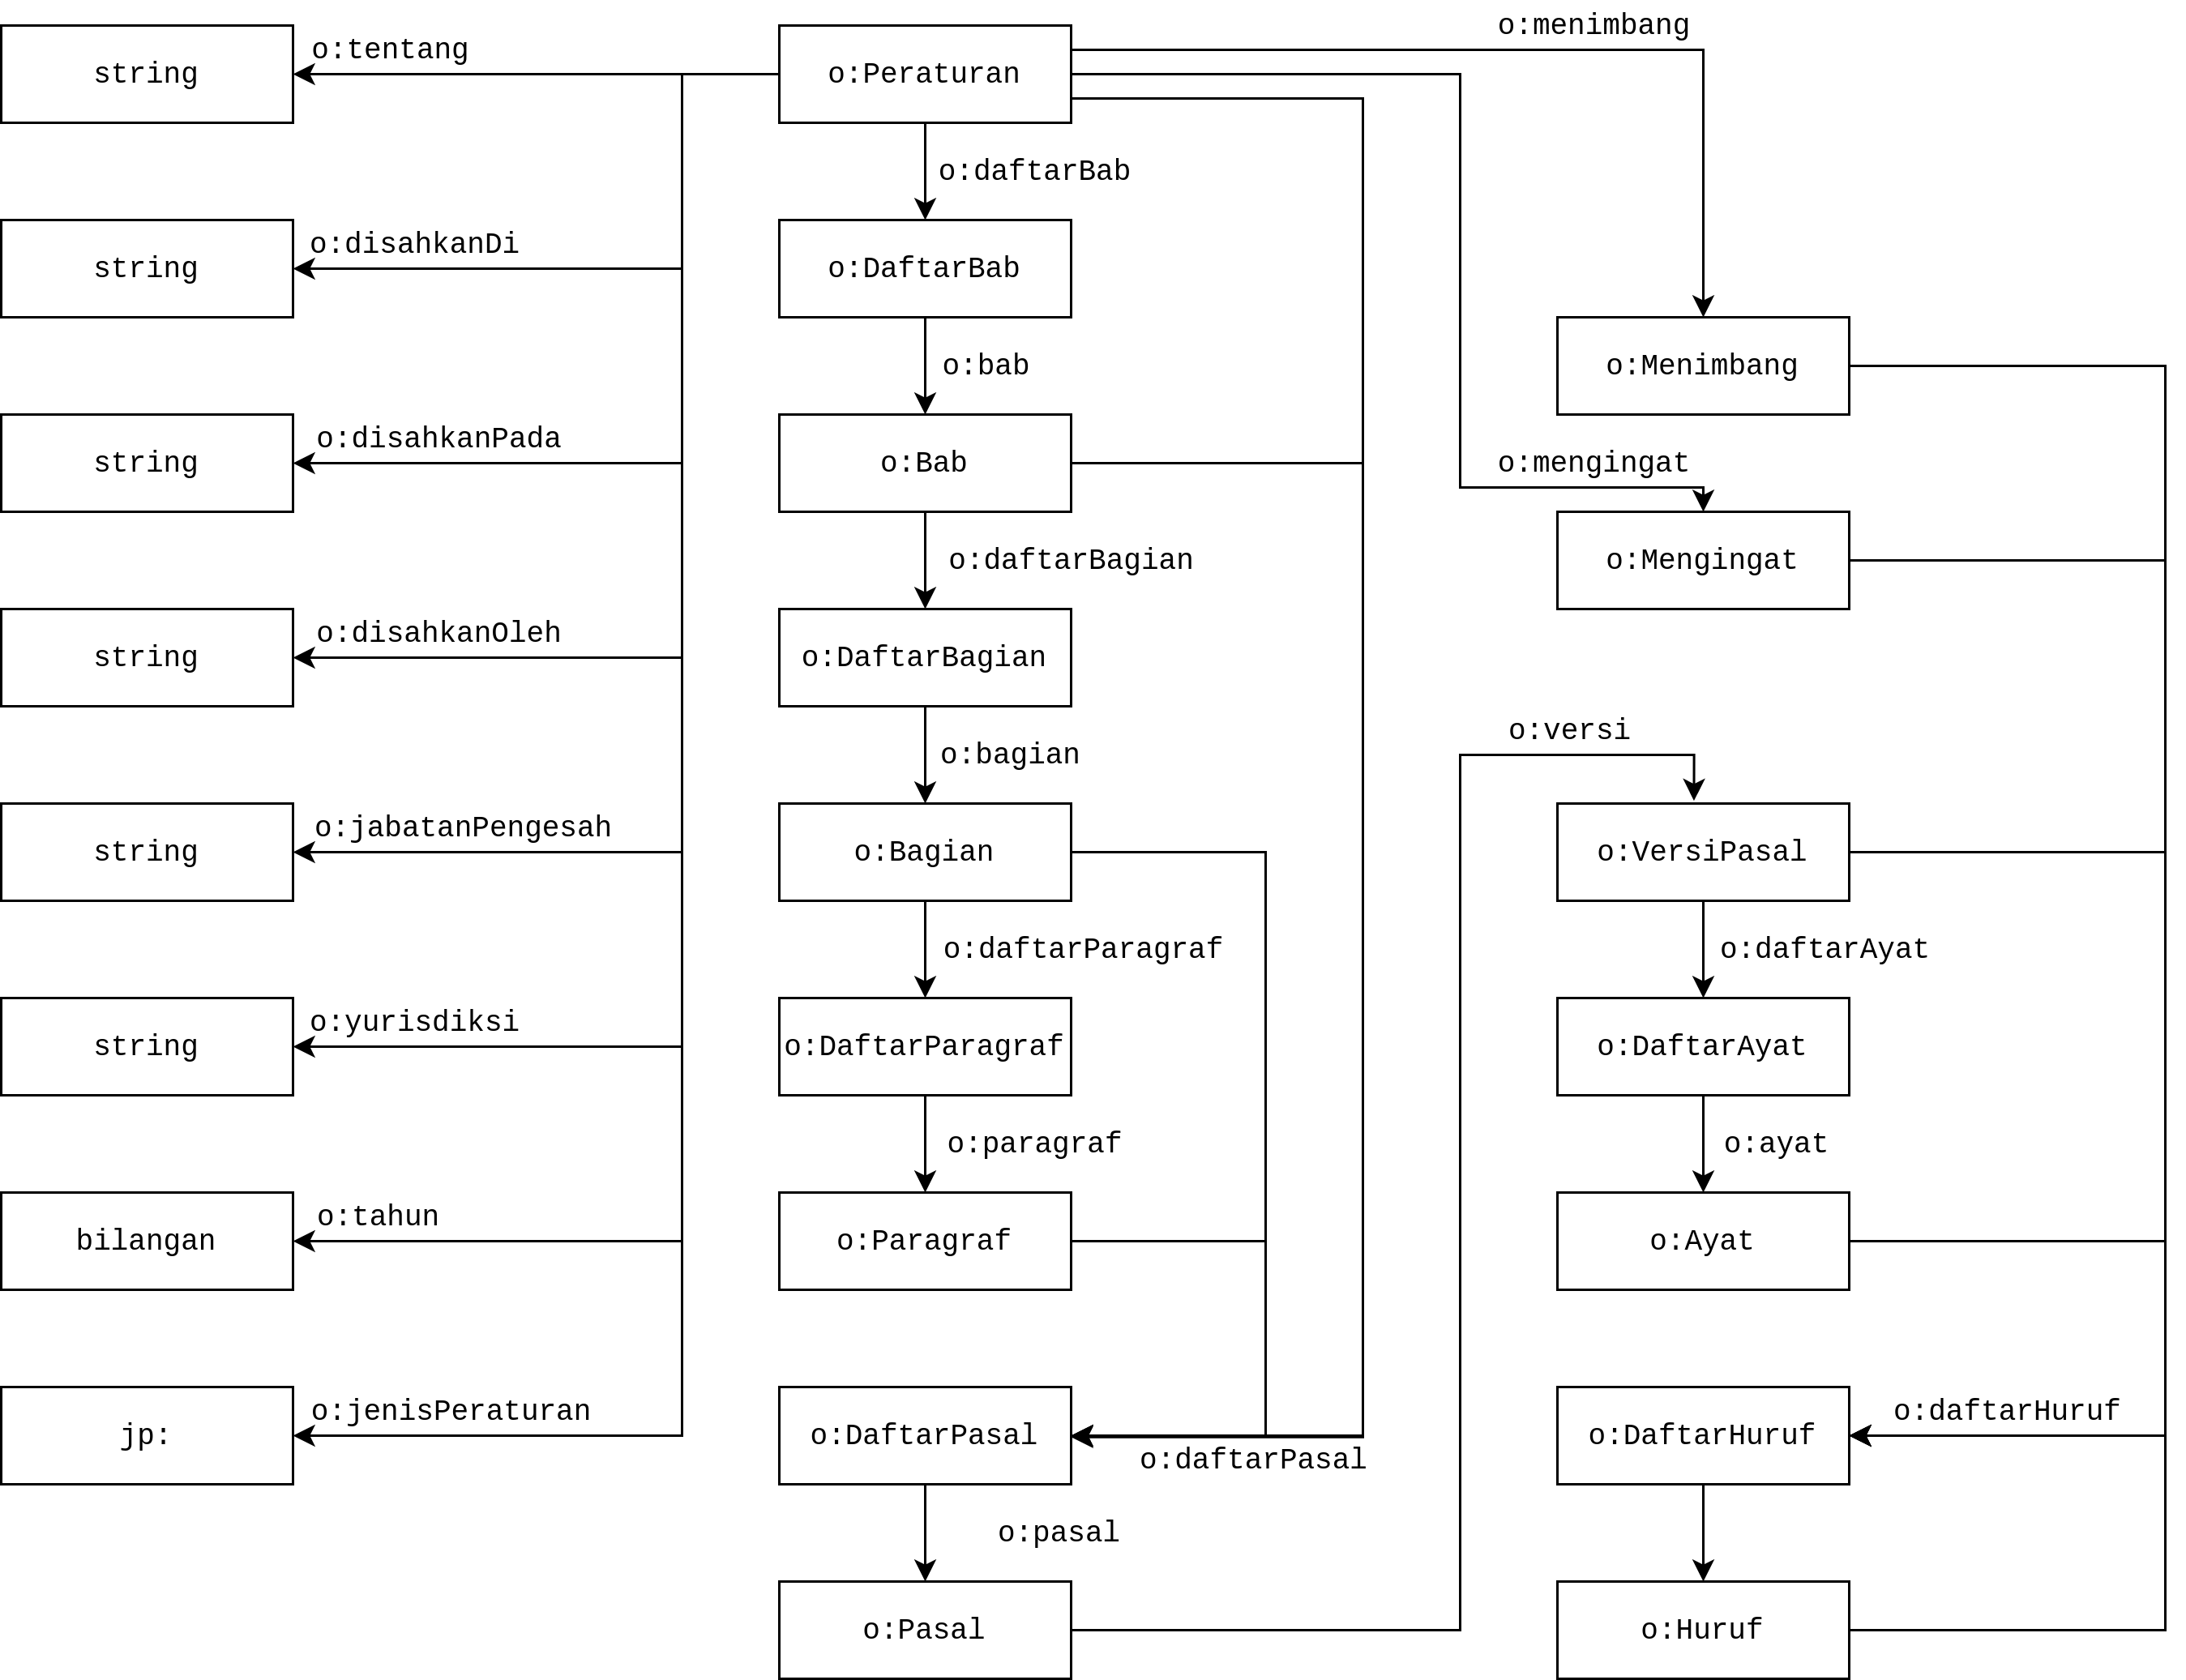
\includegraphics[width=\textwidth]{pictures/ontologi-stuktur.png}
  \caption{Ontology dari metadata dan struktur peraturan}
  \label{fig:ontologi-struktur}
\end{figure}

\pic~\ref{fig:insert}, \pic~\ref{fig:insert}, dan \pic~\ref{fig:insert} memuat ontologi untuk
amendemen peraturan. Setiap terjadi perubahan, akan ditambahkan \mono{VersiPasal} baru. Dengan
ontologi ini, dapat dilakukan \textit{query} untuk mengambil versi terakhir dari pasal untuk dilihat
statusnya apakah orisinal, telah dihapus, hasil pengubahan, atau hasil penyisipan.

\begin{figure}[H]
  \centering
  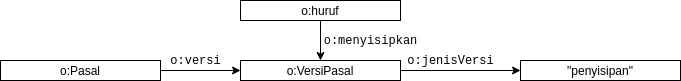
\includegraphics[width=\textwidth]{pictures/insert.png}
  \caption{Ontology penyisipan peraturan}
  \label{fig:insert}
\end{figure}

\begin{figure}[H]
  \centering
  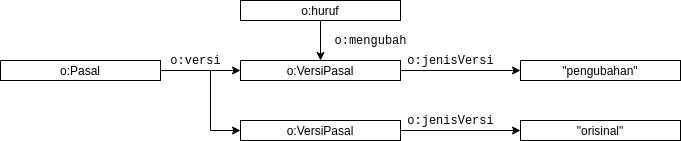
\includegraphics[width=\textwidth]{pictures/update.png}
  \caption{Ontology pengubahan peraturan}
  \label{fig:update}
\end{figure}

\begin{figure}[H]
  \centering
  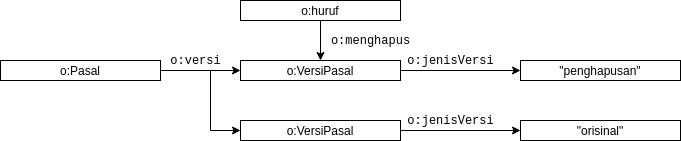
\includegraphics[width=\textwidth]{pictures/delete.png}
  \caption{Ontology penghapusan peraturan}
  \label{fig:delete}
\end{figure}
